%!TEX root = report.tex
\section{Teknisk utførelse}\label{sec:teknisk}
Denne seksjonen vil detaljere hvordan Garbage Alert per i dag er
implementert, samt tanker om videre utvikling til en eventuell ferdig
versjon.
\subsection{Tidlig prototype}
Tidlig i prosessen ble det utviklet en enkel web-basert prototype som
kunne brukes for å utforske spillets dynamikk. Denne var hjelpsom for å
fastslå hvilke deler av konseptet som fungerte, og ikke fungerte. Se
figur~\ref{fig:screenshot_tidlig_prototype}, under for et skjermskudd av
denne prototypen. Et mål var å ha noe som fungerte, men samtidig
realisere den med minimal bruk av tid.
\begin{figure} [H]
	\begin{center}
	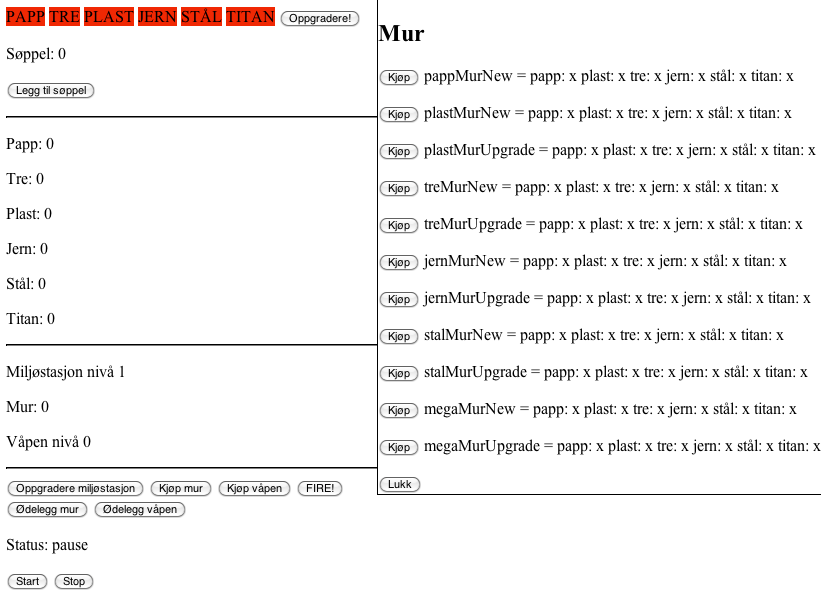
\includegraphics[scale=0.3]{images/screenshot_tidlig_prototype.png}
	\end{center}
	\caption{Skjermskudd av vår tidlige prototype}
	\label{fig:screenshot_tidlig_prototype}
\end{figure}

Denne programkoden, sammen med penn, papir og en solid dose fantasi
gjorde oss i stand til å spille spillet sammen på et veldig tidlig
stadie, noe som gjorde oss i stand til å gjøre nødvendige justeringer
for å gjøre spillet morsommere å spille. Vi kunne og gjøre et bedre
anslag på spillets ressurskostnader og
nedkjølinger\footnote{Nedkjølinger er et ord som benyttes om den tiden
det tar fra du utfører en handling til du får lov til å utfører den
igjen.}.

Denne prototype-koden ble og senere mye brukt, sammen med en bedre grafisk presentasjon, for å realisere den endelige protoypen.



\subsection{Endelig prototype}

Garbage Alert-prototypen slik den er i dag er implementert med de nye
web-teknologiene (noe unøyaktig) kjent som HTML5. Mer nøyaktig vil dette si at spillet er implementert med et \texttt{<canvas>} element, et lite "malebrett" som en kan tegne på programmatisk med JavaScript. Dette medfører at Garbage Alert i prinsippet kan kjøres hvor som helst der en har en moderne nettleser med støtte for JavaScript. Garbage Alert har moderne berøringsbaserte mobiltelefoner som hovedplattform, hvor slik teknologi kjører uten problemer.





Enkelte av elementene er dog implementert via andre ymse metoder, som for eksempel hvite overlegg som ser litt malplassert ut i forhold til resten av grensesnittet, grunnet gjenbruk av kode fra en tidligere prototype, for å raskt kunne iterere og skape en prototype vi kunne teste ut og vise fram. Dette ville i en ferdig versjon blitt implementert på en skikkelig måte.


\subsubsection{Systemkrav}
Som nevnt over er Garbage Alert først og fremst ment å kunne spilles på mobiltelefoner.
Da spillet er implementert som et web-basert spill vil det i prinsippet ikke være en begrensning på hvilket operativsystem telefonen kjører, det være Apple iOS, Google Android eller Windows Phone 7, så lenge telefonen leveres med en moderne nettleser. Nettbrett som Apple iPad og Samsung Galaxy Tab vil og kunne kjøre Garbage Alert.

I tillegg til dette vil spillet kunne spilles ellers hvor der finnes moderne/kompatible nettlesere. Det store aberet her er at kontrollmetoder ikke alltid vil fungere optimalt, og må eventuelt tilpasses de ulike plattformers styrker og svakheter. Slik prototypen eksisterer i dag vil den eksempelvis fungere bra med mus og tastatur på en tradisjonell datamaskin, men ikke i det hele tatt med en styrespak.

Legg dog merke til at ekstensiv testing av ulike nettlesere og enheter har ikke blitt gjort, og gruppen kan ikke gå god for at spillet kjører feilfritt over alt. Garbage Alert er hovedsaklig testet i Google Chrome (versjon 18 og over) og Opera (versjon 11.6 og over). Spillet har blitt testet noe på mobiltelefoner, men ikke ut over det å sikre at spillet fungerer \emph{greit}. I en endelig versjon må grensesnittet tilpasses bedre, og ekstensiv testing måtte vært utført for å sikre at spillet fungererer skikkelig.


\subsubsection{Audiovisuelt innhold}
Garbage Alerts visuelle stil er ment å være leken og samtidig
oversiktlig, og dets grafiske stil er inspirert av den klassiske
spillserien Advance Wars.

Spillets introskjerm er ment å være så pompøs og lite subtil som mulig,
med store eksplosjoner på en søppelhaug. På denne skjermen spilles et
utsnitt av sangen \emph{Hell March}, kjent som tittelmusikken fra
Westwoods Red Alert-serie. Dette for å underbygge det pompøse inntrykket
vi ønsker å skape. En ferdig versjon vil inneholde lydeffekter og
bakgrunnsmusikk i resten av spillet.

En mer fullstendig utdyping av spillets audiovisuelle innhold finnes i
seksjon \ref{sec:artwork}.



\subsubsection{Programmeringsinnhold og kodestruktur}
Som nevnt over er spillet programmert i JavaScript fra grunnen av uten hjelp av eksisterenede hjelperammeverk. Dette er dels fordi implementasjonen av spillet er tenkt å være enkel, samt at slike rammeverk er noe umodne.
Logisk kodestruktur og -arkitektur har ikke vært noe som har blitt tenkt mye på, og kun enkle grep har blitt gjort for å gjøre koden noe enklere å skrive. Dette gjelder spesielt den koden som har blitt arvet fra den tidligere prototypen, kode som med god grunn kan omtales som et "lappeteppe".

For å øke spillets modifiserbarhet og øke kodens lesbarhet er de ulike elementene i spillet delt inn i egne JavaScript-filer for å logisk samle metoder og funksjoner. I en ferdig versjon vil disse filene samles i én enkelt fil for å gjøre eksempelvis innlastingstiden bedre.

Spillets bilder og figurer finnes i en egen mappe. På samme måte som med JavaScript-filene vil en i den ferdige versjonen ha salle bildene i én større bildefil for å forbedre innlastingstiden.


\subsubsection{Problemer og alternativer}
Da vi har sett oss ut berøringsbaserte mobiltelefoner som målplattform for spillet vil de naturlige alternativene være å realisere Garbage Alert som en såkalt \emph{native} applikasjon\footnote{En \emph{native} applikasjon er en skreddersydd applikasjon skrevet direkte til ett enkelt av de ulike mobiltelefonoperativsystemene.}, noe vi også til å begynne med hadde tenkt å gjøre. Dette gikk vi imidlertid bort fra da ikke alle har de verktøy som behøves for å utvikle til denne plattformen\footnote{Der behøves en Apple Mac og en utviklerlisens, noe kun ett menneske på gruppa har.} falt valget med hvert på å implementere spille med web-teknologi. Dette førte med seg at flere kunne bidra til programmeringen både i kraft av at flere har erffaring med JavaScript fra før og at alle er i besittelse av de verktøy som behøves.

Spill skrevet i JavaScript vil være tregere enn spill skrevet native, men dette er noe vi har valgt å se bort fra. Dette fordi en enkel prototype vil fungere tilstrekkelig i dette prosjektet.

Det som nevnt ingen garanti at spillet vil fungere i alle nettlesere overalt, og ekstensiv testing må til for å kunne sikre at det fungerer på flest mulig enheter. Igjen, grunnet at resultatet av dette prosjektet var ment å kun være en enkel prototype, er dette noe vi har sett bort fra.

Flerspiller-delen av spillet har ikke blitt implementert, ei heller en kunstig intelligens til motspilleren.


\subsubsection{Ressurser}
Garbage Alert kan utvikles i hvilken som helst applikasjon som er i stand til å redigere rene tekstfiler. Kildekontroll gjøres via Git, og koden er lagret på GitHub\footnote{\url{https://github.com/aspic/Garbage-Alert}}. Spillet kan og spilles fra spillet nettside på \url{http://aspic.github.com/Garbage-Alert}.

\subsubsection{Hvordan spille Garbage Alert lokalt}
Forutsett at du har Git og Python\footnote{Hvilken som helst server-programvare kan benyttes, Python nevnes her da dette verktøysettet er temmelig utbredt og er enkelt å starte.} installert, her er hvordan du starter spillet fra egen datamaskin via en terminalklient.

Først, last ned kildefilene fra GitHub med kommandoen \newline\texttt{git clone git://github.com/aspic/Garbage-Alert.git}. Spillet vil da lastes ned til mappen \texttt{Garbage-Alert}. Navigér til mappa kalt \texttt{webver} under denne  og start spillet med kommandoen \texttt{python -m SimpleHTTPServer 8080}. Start en kompatibel nettleser og navigér til URLen \url{http://localhost:8080}. Garbage Alert vil nå kjøre lokalt på din datamaskin.
